%%%%%%%%%%%%%%%%%%%%%%%%%%%%%%%%%%%%%%%%%
% Beamer Presentation
% LaTeX Template
% Version 1.0 (10/11/12)
%
% This template has been downloaded from:
% http://www.LaTeXTemplates.com
%
% License:
% CC BY-NC-SA 3.0 (http://creativecommons.org/licenses/by-nc-sa/3.0/)
%
%%%%%%%%%%%%%%%%%%%%%%%%%%%%%%%%%%%%%%%%%

%----------------------------------------------------------------------------------------
%	PACKAGES AND THEMES
%----------------------------------------------------------------------------------------

\documentclass{beamer}

\mode<presentation> {

% The Beamer class comes with a number of default slide themes
% which change the colors and layouts of slides. Below this is a list
% of all the themes, uncomment each in turn to see what they look like.

%\usetheme{default}
%\usetheme{AnnArbor}
%\usetheme{Antibes}
%\usetheme{Bergen}
%\usetheme{Berkeley}
%\usetheme{Berlin}
%\usetheme{Boadilla}
%\usetheme{CambridgeUS}
%\usetheme{Copenhagen}
%\usetheme{Darmstadt}
%\usetheme{Dresden}
%\usetheme{Frankfurt}
%\usetheme{Goettingen}
%\usetheme{Hannover}
%\usetheme{Ilmenau}
%\usetheme{JuanLesPins}
%\usetheme{Luebeck}
\usetheme{Madrid}
%\usetheme{Malmoe}
%\usetheme{Marburg}
%\usetheme{Montpellier}
%\usetheme{PaloAlto}
%\usetheme{Pittsburgh}
%\usetheme{Rochester}
%\usetheme{Singapore}
%\usetheme{Szeged}
%\usetheme{Warsaw}

% As well as themes, the Beamer class has a number of color themes
% for any slide theme. Uncomment each of these in turn to see how it
% changes the colors of your current slide theme.

%\usecolortheme{albatross}
%\usecolortheme{beaver}
%\usecolortheme{beetle}
%\usecolortheme{crane}
%\usecolortheme{dolphin}
%\usecolortheme{dove}
%\usecolortheme{fly}
%\usecolortheme{lily}
%\usecolortheme{orchid}
%\usecolortheme{rose}
%\usecolortheme{seagull}
%\usecolortheme{seahorse}
%\usecolortheme{whale}
%\usecolortheme{wolverine}

%\setbeamertemplate{footline} % To remove the footer line in all slides uncomment this line
%\setbeamertemplate{footline}[page number] % To replace the footer line in all slides with a simple slide count uncomment this line

%\setbeamertemplate{navigation symbols}{} % To remove the navigation symbols from the bottom of all slides uncomment this line
}


\usepackage{booktabs} % Allows the use of \toprule, \midrule and \bottomrule in tables
\usepackage{listings}

\usepackage{minted}
\usepackage[utf8]{inputenc}
\usepackage[T2A]{fontenc}
\usepackage{amssymb, amsmath, mathrsfs, amsthm}
\usepackage[russian]{babel}
\usepackage{float}
\usepackage{pgfplotstable}
\usepackage{multirow}
\graphicspath{{./}}

%----------------------------------------------------------------------------------------
%	TITLE PAGE
%----------------------------------------------------------------------------------------

\title[Что за данные?]{Игра ``Что за данные?''} % The short title appears at the bottom of every slide, the full title is only on the title page

\author[Попов Дмитрий]{Попов Дмитрий Олегович\\
	~\\
	~\\
	~\\
	\textbf {Прикладные задачи анализа данных}\\
	~\\} % Your name
{
\medskip
}
\date{9 октября 2020 г.} % Date, can be changed to a custom date

\AtBeginSection[]
{
	\begin{frame}
		\frametitle{План}
		\tableofcontents[currentsection,currentsubsection]
	\end{frame}
}


\begin{document}

\begin{frame}
\titlepage % Print the title page as the first slide
\end{frame}

%----------------------------------------------------------------------------------------
%	PRESENTATION SLIDES
%----------------------------------------------------------------------------------------

\begin{frame}

\begin{figure}
	\centering
	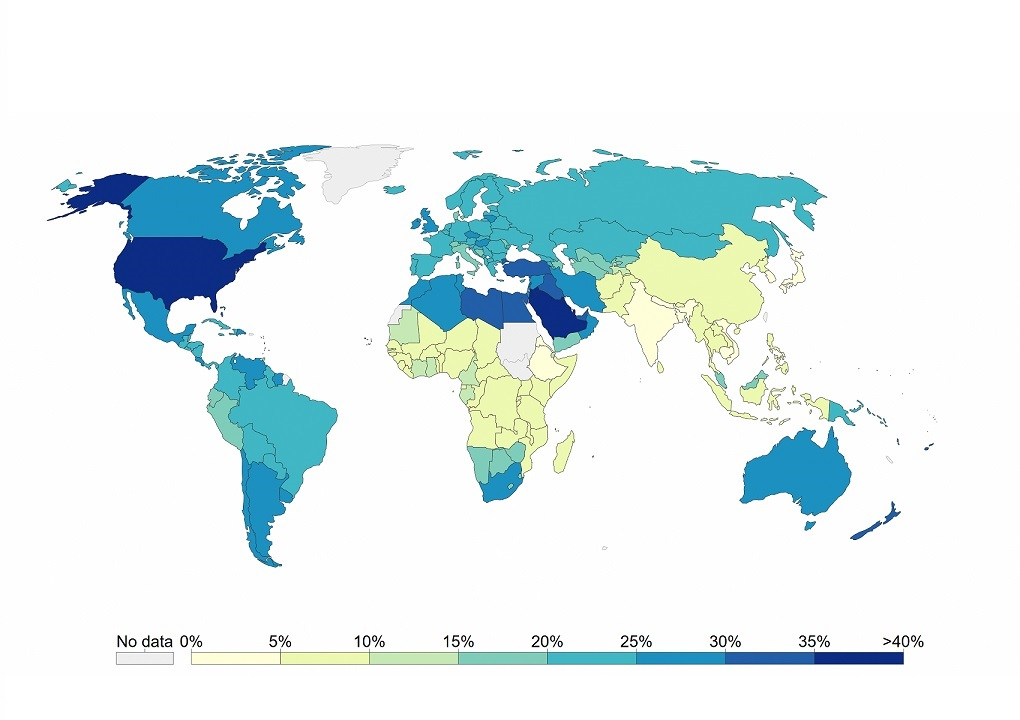
\includegraphics[width=120mm]{obese1.jpg}
\end{figure}


\end{frame}

\begin{frame}

\begin{figure}
	\centering
	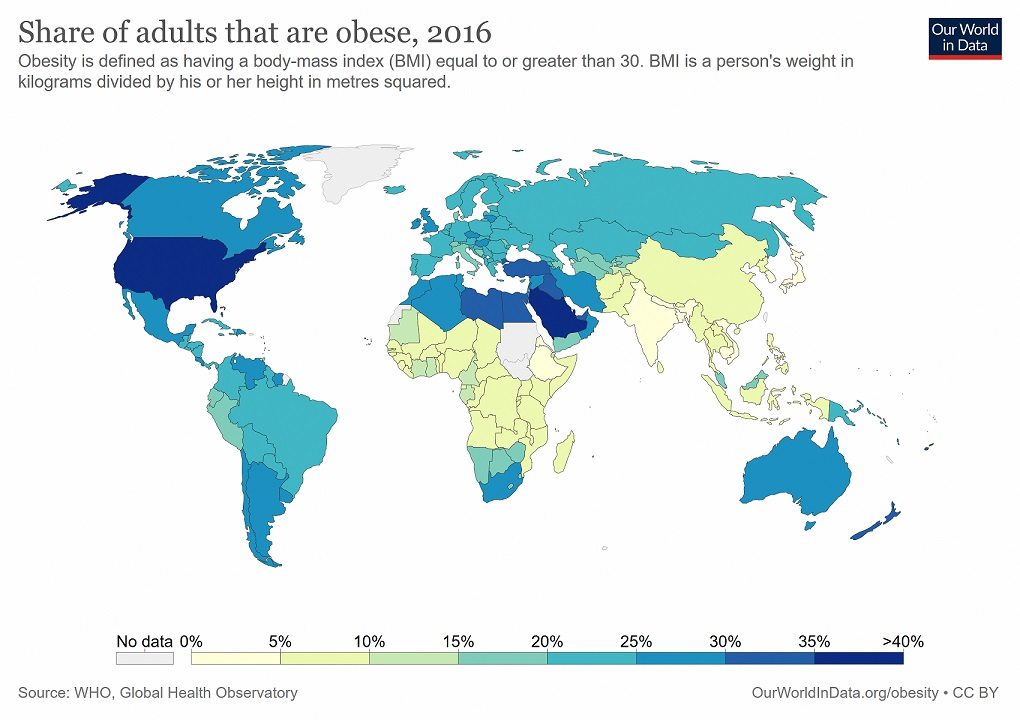
\includegraphics[width=120mm]{obese2.jpg}
\end{figure}

\end{frame}

\begin{frame}

\begin{figure}
	\centering
	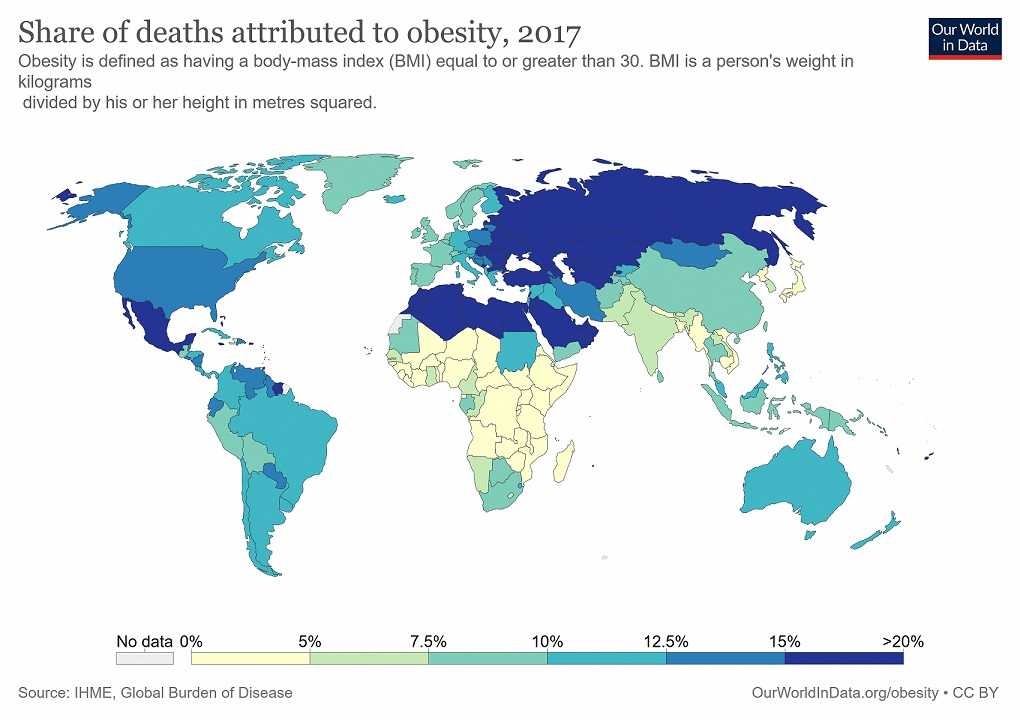
\includegraphics[width=120mm]{obese3.jpg}
\end{figure}

\end{frame}

\begin{frame}

\begin{figure}
	\centering
	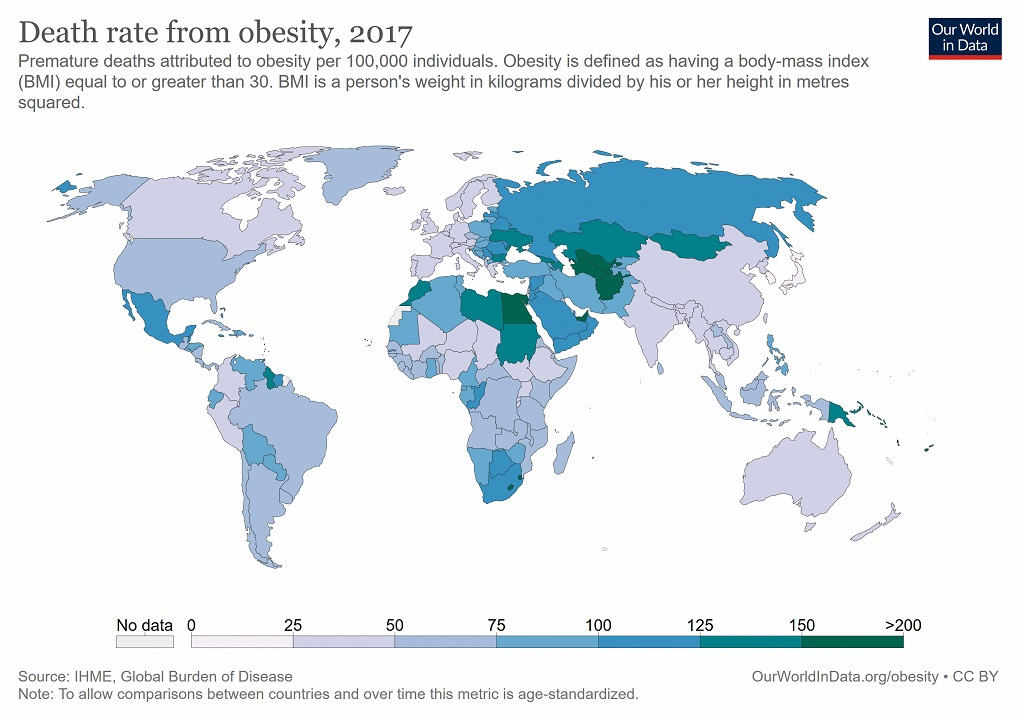
\includegraphics[width=120mm]{obese4.jpg}
\end{figure}

\end{frame}

\begin{frame}

\begin{figure}
	\centering
	\begin{minipage}{0.5\textwidth}
		\centering
		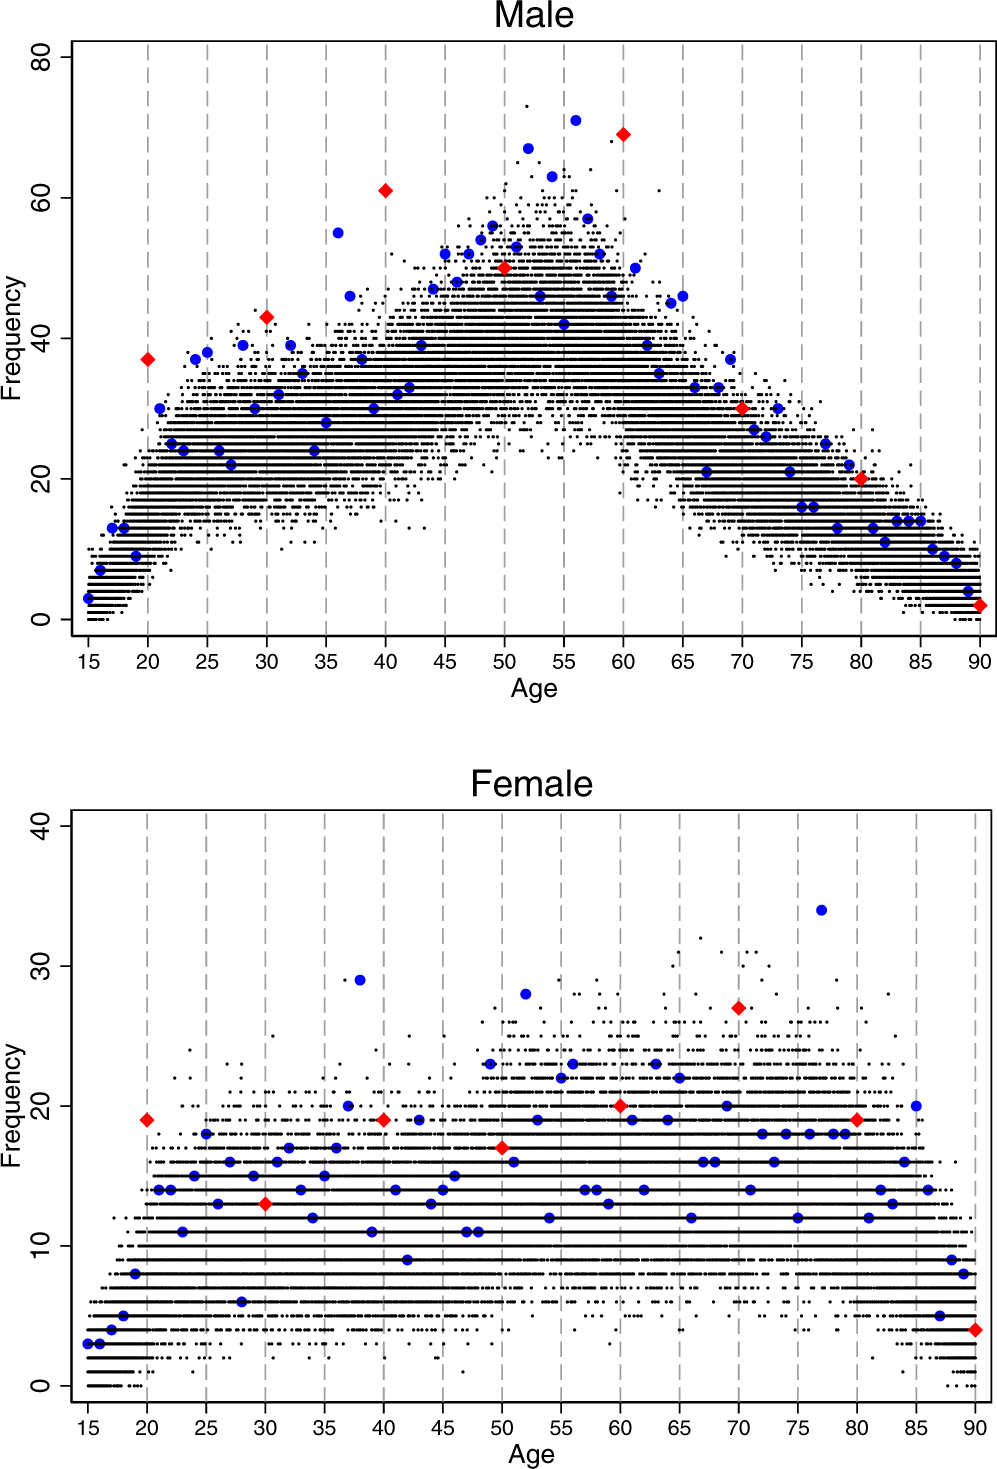
\includegraphics[width=0.9\textwidth]{suicide1.png} % first figure itself
	\end{minipage}\hfill
	\begin{minipage}{0.5\textwidth}
		\centering
		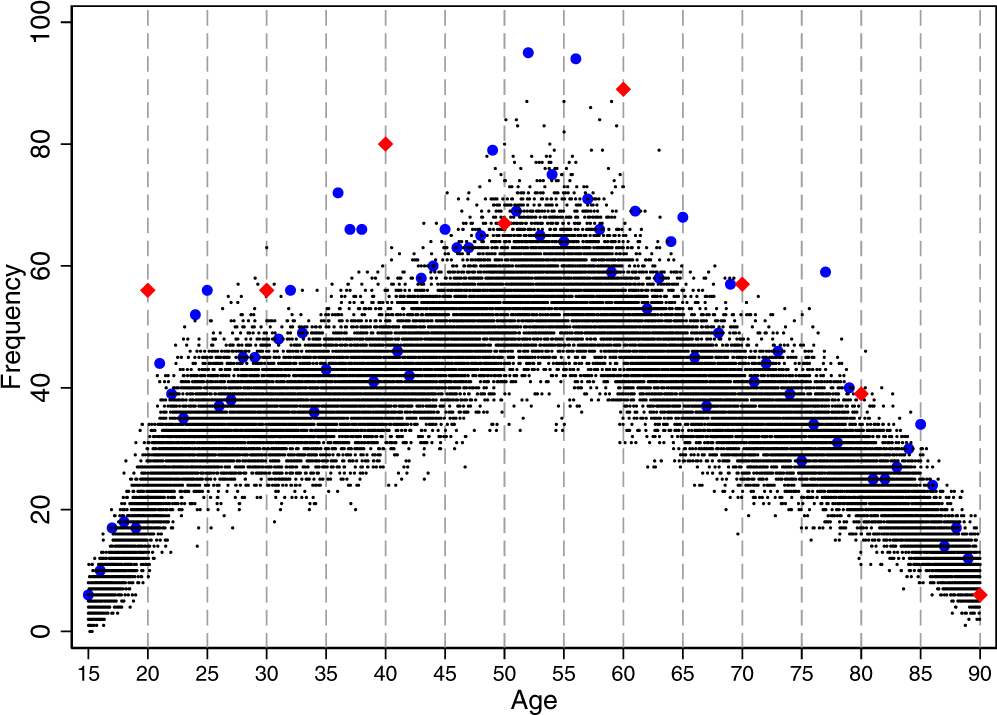
\includegraphics[width=0.9\textwidth]{suicide2.png} % second figure itself
		\caption{All population}
	\end{minipage}
\end{figure}

\end{frame}

\begin{frame}
\textbf{Higher Risk of Suicide on Milestone Birthdays: Evidence from Japan.}\\
\\
Частота самоубийств по возрасту и дате. Красные и синие маркеры обозначают частоту самоубийств в юбилейные и обычные дни рождения соответственно. Чёрные точки обозначают частоту самоубийств в остальные дни года.

\end{frame}

\begin{frame}

\begin{figure}
	\centering
	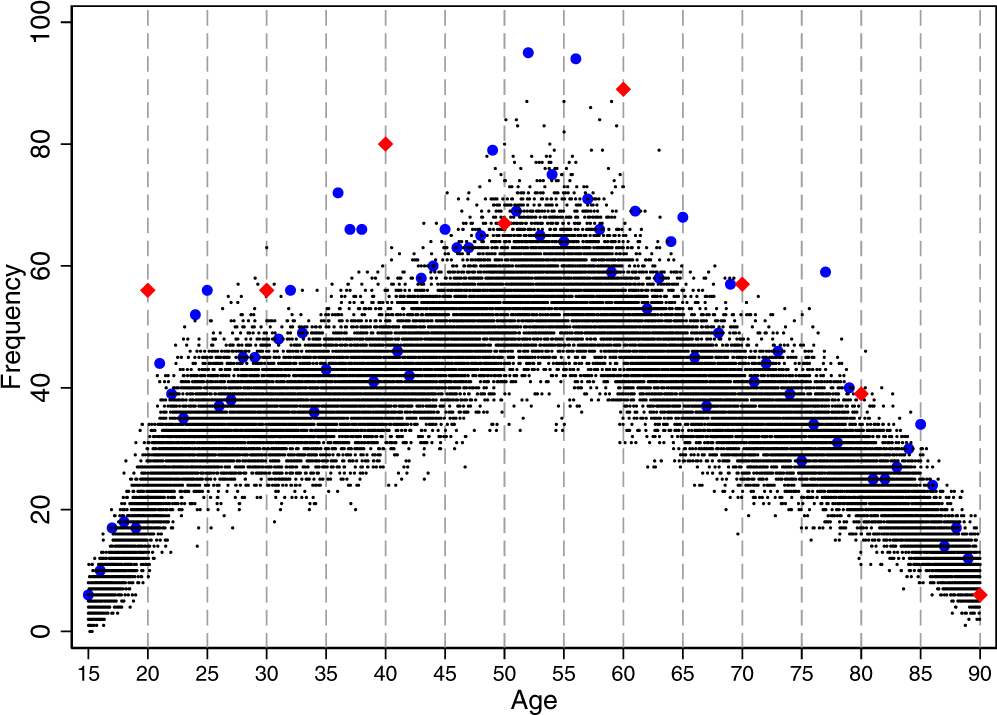
\includegraphics[width=120mm]{suicide2.png}
\end{figure}

\end{frame}

\begin{frame}

\begin{figure}
	\centering
	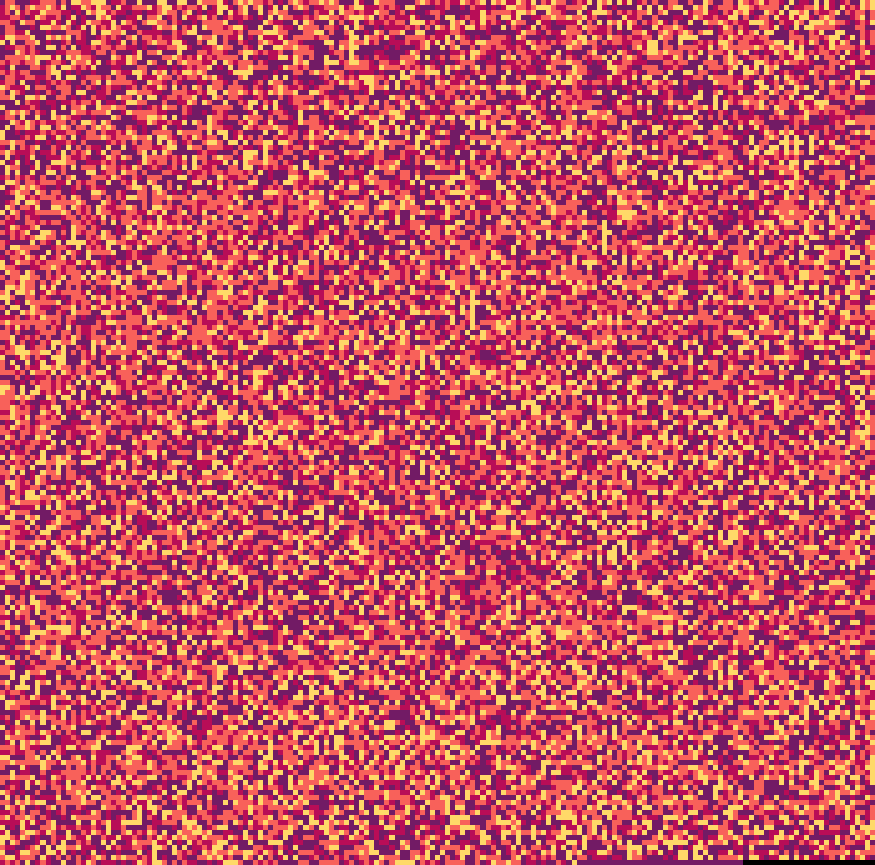
\includegraphics[width=90mm]{coronavirus.png}
\end{figure}

\end{frame}

\begin{frame}{Источники}
Статистика по ожирению:\\
$\bullet$   https://ourworldindata.org/obesity\\
\\
Статистика по самоубийствам в Японии:\\
$\bullet$   https://www.nature.com/articles/s41598-019-53203-4\\
\\
РНК коронавируса:\\
$\bullet$   https://www.reddit.com/r/dataisbeautiful/comments/fkwova/
\end{frame}

\end{document}